\documentclass[10pt,twocolumn,letterpaper]{article}

\usepackage[margin=0.75in,columnsep=0.3in]{geometry}
\usepackage{amsmath}
\usepackage{fontspec}
\usepackage{unicode-math}
\setmainfont{texgyretermes}[
  Extension=.otf,
  UprightFont=*-regular,
  BoldFont=*-bold,
  ItalicFont=*-italic,
  BoldItalicFont=*-bolditalic]
\setmathfont{texgyretermes-math.otf}
\setmonofont{Inconsolatazi4-Regular.otf}[
  BoldFont=Inconsolatazi4-Bold.otf,
  Scale=MatchLowercase]
\usepackage{microtype}
\usepackage{graphicx}
\usepackage{dblfloatfix}
\usepackage{booktabs}
\usepackage{tabularx}
\usepackage{enumitem}
\usepackage{titlesec}
\usepackage[font=small,labelfont=bf,labelsep=period]{caption}
\usepackage{xcolor}
\usepackage{listings}
\usepackage{balance}
\usepackage{needspace}
\usepackage{url}
\usepackage[colorlinks,linkcolor=linkblue,urlcolor=linkblue]{hyperref}

\definecolor{linkblue}{rgb}{0.10,0.27,0.55}
\definecolor{codebg}{RGB}{243,245,248}
\definecolor{coderule}{RGB}{208,213,221}
\definecolor{codecomment}{RGB}{110,118,129}
\graphicspath{{figures/}{../}}
\DeclareUrlCommand\code{\urlstyle{tt}\def\UrlBreaks{\do\/}\def\UrlBigBreaks{}}
\raggedbottom

\titleformat{\section}{\normalfont\large\bfseries}{\thesection}{0.6em}{}
\titlespacing*{\section}{0pt}{2.2ex plus 0.6ex minus 0.3ex}{1ex plus 0.2ex}
\setlist{itemsep=0.3ex,topsep=0.6ex,leftmargin=1.3em}
\captionsetup[table]{position=top,skip=4pt}
\captionsetup[figure]{skip=6pt}
\renewcommand{\abstractname}{Summary}
\renewcommand{\dbltopfraction}{0.85}
\renewcommand{\dblfloatpagefraction}{0.85}
\setcounter{dbltopnumber}{2}
\setlength{\dbltextfloatsep}{14pt plus 2pt minus 3pt}
\setlength{\dblfloatsep}{14pt plus 2pt minus 3pt}

\lstset{
  basicstyle=\ttfamily\small,
  backgroundcolor=\color{codebg},
  frame=single,
  rulecolor=\color{coderule},
  framesep=7pt,
  xleftmargin=7pt,
  xrightmargin=7pt,
  aboveskip=10pt,
  belowskip=10pt,
  columns=fullflexible,
  keepspaces=true,
  breaklines=true,
  morecomment=[l]{\#},
  commentstyle=\color{codecomment},
}

% A figure from reports/figures with its headline and source note cropped off, since the
% caption carries the message. Arguments: width, bottom and top crop in pixels (200 dpi), file.
\newcommand{\plot}[4]{%
  \includegraphics[width=#1,trim={0 {\dimexpr#2bp*36/100\relax} 0 {\dimexpr#3bp*36/100\relax}},clip]{#4}}

\begin{document}

\twocolumn[
\begin{@twocolumnfalse}
  \begin{center}
    {\LARGE\bfseries Freight Rate Prediction\par}
    \vspace{0.5em}
    {\large Spotter Machine Learning Engineer assessment\par}
    \vspace{0.7em}
    {Mustafa Abbas\quad\textperiodcentered\quad 25 October 2026\par}
  \end{center}
  \vspace{0.3em}
  \begin{abstract}
  \noindent Spotter asked for a model that predicts the posted rate of a freight load from its lane, distance, equipment, weight, date and two market signals. There are 48,000 loads with known prices from January to October 2025. The loads to price are 12,000 from November and December 2025, plus one fixed Lexington to Fort Wayne load priced for every day of December.

  Every load to price comes after every load with a known price, so I treated this as a forecasting problem: validate on the future, and pick a model that carries trends forward. Before modelling I took out 677 posted rates (1.4\%) that are scaled up or down by a factor of 2 to 6, and fixed the smaller problems: sign-flipped and capped weights, and missing values. Every modelling choice was made on four walk-forward folds inside January--August, each predicting the following two months. September--October stayed untouched until a single final test.

  The final model is a regularised linear regression on log price. Its inputs follow what the data showed: smooth curves for distance and weight, the market index, a steady upward drift, city effects, lane effects (a lane being a pickup city and delivery city pair), and a quarter-end price surge that is about three times larger for flatbeds than for dry vans. On the September--October test its average error is 1.41\%, against 1.70\% for a plain linear regression baseline (about \$33 vs \$39 per load), close to the 1.37\% the folds had predicted. Gradient-boosted trees, a random forest and a neural network all did worse, mainly because they can't carry the upward drift past their training dates.

  Submitted with this report: \code{validation_predictions.csv} for all 12,000 loads, the filled December chart inputs, and the code. The repo README has the two commands that reproduce both. The December chart and what drives its shape are in Section~\ref{sec:december}.
  \end{abstract}
  \vspace{0.6em}
  \noindent\rule{\textwidth}{0.4pt}
  \vspace{1.2em}
\end{@twocolumnfalse}
]

\section{Data and data quality}\label{sec:data}

The labelled file has 48,000 loads covering every day from 1~January to 31~October 2025 (115 to 198 a day), with three equipment types and 64 cities. A lane is a route from one pickup city to one delivery city, so Lexington to Fort Wayne and Fort Wayne to Lexington are different lanes. The data covers 4,014 of the 4,032 possible lanes, with about 10 loads on a typical lane. About 6\% of loads carry at least one problem. None of the problems cluster in a particular month, so they look like recording errors rather than real market behaviour.

Corrupted prices are the one that matters most. 677 posted rates (1.4\%) are off by a factor of 2 to 6, roughly half too high and half too low (Figure~\ref{fig:corruption}). To find them I compared each price with what comparable loads cost (same distance, equipment, weight, cities, market index and date). Every other load lands within 0.92--1.11$\times$ of that expected price, and there is nothing in between, so a simple rule separates them cleanly: anything more than 1.5$\times$ above or below expected is flagged. The rule is refitted inside each training window, and it flags exactly the same 677 loads every time. Left in, these rows would drag any model towards prices that never existed, and they would also make the error scores meaningless.

\begin{figure*}[t]
  \centering
  \plot{\textwidth}{54}{225}{eda/02_label_corruption.png}
  \caption{1.4\% of posted rates are off by a factor of 2--6, with nothing in between. Left: posted rate against distance, with the 677 flagged loads in orange. Right: each price divided by its expected price, the typical cost of loads with the same distance, equipment, weight, cities, market index and date. Normal loads sit within 0.92--1.11$\times$; flagged loads are 2.3--5.8$\times$ too low or 2.2--5.3$\times$ too high.}
  \label{fig:corruption}
\end{figure*}

The rest were simpler:
\begin{itemize}
  \item 292 negative weights are sign flips. Their absolute values price exactly like normal weights (Figure~\ref{fig:weight}), so I flipped them. 1,204 loads sit at exactly 47,500\,lb, a recording cap. They price like the heaviest uncapped loads, so I kept them with a flag.
  \item 374 missing market index values are filled from other loads on the same day, since the index is mostly a daily number, and 300 missing weights get the training median. Both get a flag.
  \item \code{quote_signal} isn't missing, but it is unreliable. Its link to price switches on and off from month to month: clearly positive in some months, absent in others, reversed in October. It has no link to the corrupted prices either (they are equally common at every level of the signal), so it isn't leaking information about the label. I left it out of the model; Section~\ref{sec:validation} explains how its instability showed up.
\end{itemize}

\begin{figure*}[t]
  \centering
  \plot{\textwidth}{55}{190}{eda/03_weight.png}
  \caption{Negative weights are sign flips. Left: recorded weights, with 292 negative values, 32 loads at the 5,000\,lb floor and 1,191 at the 47,500\,lb cap (13 more sit at $-$47,500\,lb). Right: price against weight, compared with similar loads. Flipped negative weights fall on the same S-shaped curve as positive ones, and capped loads price like the heaviest uncapped loads.}
  \label{fig:weight}
\end{figure*}

All fixes are learned from the training rows only and applied the same way to anything the model predicts, including Spotter's 12,000 loads (which had 145 sign flips, 165 missing weights and 249 missing index values of their own).

\section{What drives the price}\label{sec:drivers}

Once the bad labels are out, prices are very regular. Distance does most of the work: on its own it explains 99\% of the variation in log price. Pricing looks like a fixed charge of about \$250--280 plus \$1.75--2.00 a mile, so short hauls cost more per mile. Equipment adds a constant percentage at every distance (Reefer about +13\% and Flatbed about +8\% over Dry Van), and weight adds up to about 8\% on an S-shaped curve. The pickup and delivery cities shift the price by up to $\pm$4\%, and a lane carries a small effect of its own, under 1\%, on top of its two cities. Figure~\ref{fig:drivers} shows how much each of these adds.

\begin{figure*}[t]
  \centering
  \plot{0.8\textwidth}{110}{215}{eda/12_what_drives_price.png}
  \caption{Distance alone prices a load to within about 7\%, and the other factors bring that down to about 2\%. Each bar is the typical unexplained variation (standard deviation of log price) after adding that factor to a simple linear fit. Knowing nothing about a load, the typical spread is 65\%.}
  \label{fig:drivers}
\end{figure*}

The rest is time (Figure~\ref{fig:time}). The market index moves the overall price level: it climbs through the spring, steps up in mid-April and down in late July, and has a weekly cycle that is high mid-week and low at the weekend. Two patterns remain once it is taken out. Prices drift upward by about 0.6\% a month, and they rise over the last five weeks of every quarter, faster towards the last day, then reset. After all of this, about 1.8\% of each price is left unexplained, the same share at every distance. That noise is the floor for any model's error.

\begin{figure*}[t]
  \centering
  \plot{0.78\textwidth}{50}{190}{eda/08_price_over_time.png}
  \caption{The market index explains the big seasonal swing; a steady drift and quarter-end spikes remain. Top: the daily price level of a standard load (distance, equipment, weight and cities taken out), relative to the period average. Middle: the market index, averaged by day. Bottom: the price level once the market index is also taken out, with the drift (+6.1\% over ten months) as a straight line. Shaded: the last five weeks of each quarter.}
  \label{fig:time}
\end{figure*}

\section{Validation and split}\label{sec:validation}

I validated the model the way it will be used: train on the past, predict the next two months. Spotter's loads all come after the labelled data, and prices in this data drift upward over time and follow the calendar (Section~\ref{sec:drivers}). A random split would let the model learn from the days around every load it is scored on, which flatters it and hides anything that stops working over time.

So the labelled months are split by date (Figure~\ref{fig:scheme}):
\begin{itemize}
  \item Four walk-forward folds sit inside January--August. Each trains on everything up to a cut-off and is scored on the following two months: April--May, May--June, June--July and July--August. Two months matches the length of Spotter's set. Every modelling choice (features, settings, which model) was made on the average of these four.
  \item September--October is a one-time test, held back from the start and scored once, after the model was fixed. September also ends a quarter, like December, so the test includes a quarter-end price surge.
  \item The final model is retrained on all ten months before predicting November--December, so holding back the test costs nothing in the end.
\end{itemize}

\begin{figure*}[t]
  \centering
  \plot{0.9\textwidth}{80}{240}{validation/validation_scheme.png}
  \caption{Every check trains on the past and predicts the next two months. The four folds' average drove every modelling choice. September--October is scored once at the end, and the final model trains on all ten months before predicting Spotter's loads. Numbers are loads in each period, before corrupted prices are removed.}
  \label{fig:scheme}
\end{figure*}

Corrupted prices are removed from training and from scoring in every split; no model should be judged on a typo.

The error measure is MAPE, the average percentage error:
\begin{equation}
  \text{MAPE} = \frac{1}{n}\sum_{i=1}^{n}\left|\frac{\hat{y}_i - y_i}{y_i}\right|,
\end{equation}
where $y_i$ is the posted rate and $\hat{y}_i$ the prediction. The unexplained part of a price is about the same percentage at every distance (roughly 1.8\%), so dollar errors grow with trip length. A percentage measure treats a \$300 short haul and a \$6,000 cross-country load the same way. I report the dollar error (mean absolute error) alongside it.

This setup ended up changing the model, not just the scores. During development, a model that used \code{quote_signal} looked harmless on a random split of January--August: its error was 1.22\% with or without it. On the walk-forward folds it fell apart. Trained on January--March, when \code{quote_signal} rose along with prices, the model learned to lean on it. In April--May the signal's level dropped and its link to price vanished (Figure~\ref{fig:signals}, right) while prices held up, so the model under-priced those months by about 7\%. Its error was 11.7\%, against 1.4\% without \code{quote_signal}. The random split also put the final model's error at 1.22\%, against 1.37\% on the walk-forward folds, which is exactly the kind of optimism I wanted to avoid.

\begin{figure*}[t]
  \centering
  \plot{\textwidth}{55}{225}{eda/10_market_signals.png}
  \caption{\texttt{market\_index} carries strong price information; \texttt{quote\_signal}'s link to price switches on and off. Left and middle: loads sorted into ten equal groups by each signal, against their price compared with similar loads. Right: the same-day correlation between \texttt{quote\_signal} and price, month by month.}
  \label{fig:signals}
\end{figure*}

\section{Model}\label{sec:model}

I compared two models, both trained on log price. The baseline is a plain linear regression on the cleaned features as they are. The final model is a ridge regression (a lightly regularised linear regression) whose inputs follow what the data showed:
\begin{equation}
  \begin{split}
    \log(\text{rate}) ={}& f(\text{distance}) + g(\text{weight}) + \beta_{\text{equip}} + \beta_{\text{mi}}\, m \\
    &+ \tau\, t + \gamma_{\text{equip}}\, r(d) + \delta_{\text{weekday}} \\
    &+ c_{\text{pickup}} + c_{\text{delivery}} + \ell_{\text{lane}} + \phi \cdot \text{flags}.
  \end{split}
  \label{eq:model}
\end{equation}
Here $f$ and $g$ are smooth curves (distance behaves like a fixed charge plus a per-mile rate; weight has an S-shaped effect), $m$ is the market index, $t$ is the date in days and $\tau$ the upward drift per day. Each $c$ is the effect of the pickup or delivery city, $\ell$ is the lane's own effect on top of its two cities, and the flags mark loads whose weight was missing or capped or whose market index was filled in. Working on the log scale turns ``Reefer costs about 13\% more'' into a single added term, and it matches how the noise behaves.

The quarter-end term needs a word. Prices start rising about five weeks before a quarter ends and accelerate into the last day, then reset. With $d$ as the days left in the quarter, the ramp is
\begin{equation}
  r(d) = \max\left(0,\ \frac{35 - d}{35}\right)^{1.5}.
\end{equation}
Its size $\gamma$ is learned separately for each equipment type, because the surge on the last day is about +2.6\% for Dry Van, +5.5\% for Reefer and +8.6\% for Flatbed (Figure~\ref{fig:learned}).

\begin{figure*}[t]
  \centering
  \plot{\textwidth}{55}{190}{model/03_what_the_model_learned.png}
  \caption{What the final model learned, fitted on January--August: rate per mile by distance for each equipment type (left), the S-shaped weight effect relative to a 30,000\,lb load (middle), and the quarter-end ramp $\gamma_{\text{equip}}\,r(d)$ (right). The distance and weight curves average the model's predictions over 3,000 real loads.}
  \label{fig:learned}
\end{figure*}

Two smaller details. Lane effects rest on about 10 loads each, so they are shrunk much harder than everything else. And Spotter's set contains eight cities that never appear in the training data (1,447 loads, e.g.\ Laredo, Chicago, Allentown). City effects follow a smooth regional pattern (Figure~\ref{fig:geography}), so a new city takes the average effect of its three nearest known cities. When I hid eight known cities on the folds to test this, error on their loads dropped from 2.08\% (pricing them as average) to 1.55\%.

\begin{figure*}[t]
  \centering
  \plot{\textwidth}{95}{190}{eda/07_geography.png}
  \caption{City effects follow a smooth regional pattern. Left: each city's effect on price, placed on the map (dot size is load volume). Loads are pricier around Oklahoma City, Houston and Dallas and cheaper around Syracuse, Albany and Buffalo. Right: a city has the same effect as a pickup and as a delivery ($r = 0.99$). Effects are measured after distance, equipment, weight, market index, month and weekday.}
  \label{fig:geography}
\end{figure*}

Why a linear model and not something heavier? I also tried gradient-boosted trees (LightGBM, XGBoost, CatBoost), a random forest and a small neural network. The tree models landed at 2.0--3.0\% on the folds and the neural network at 4.9\%, against 1.37\% (full table in Appendix~\ref{app:alternatives}). The main reason is extrapolation: a tree can't extend the upward drift past its last training date, so it under-prices the next two months, and the further ahead, the worse. A hybrid that put LightGBM on top of the final model matched it (1.36\%) but added nothing, so I kept the simpler model. A side benefit is that every effect it learned can be read and checked.

\section{Results}\label{sec:results}

The final model beats the baseline on every fold and on the held-back test, and the test lands where the folds said it would (Table~\ref{tab:results}, Figure~\ref{fig:test}).

\begin{table}[!h]
  \centering
  \small
  \caption{Average error per load. Folds: the four walk-forward folds inside January--August. Test: September--October, scored once. The dollar error is the mean absolute error.}
  \label{tab:results}
  \begin{tabular}{@{}lcccc@{}}
    \toprule
    & \multicolumn{2}{c}{Folds (Jan--Aug)} & \multicolumn{2}{c}{Test (Sep--Oct)} \\
    \cmidrule(lr){2-3}\cmidrule(l){4-5}
    Model & MAPE & \$ error & MAPE & \$ error \\
    \midrule
    Baseline & 1.73\% & \$42 & 1.70\% & \$39 \\
    Final model & \textbf{1.37\%} & \textbf{\$33} & \textbf{1.41\%} & \textbf{\$33} \\
    \bottomrule
  \end{tabular}
\end{table}

The gain isn't a handful of lucky loads: the final model is more accurate on 63\% of individual fold loads and 59\% of test loads. It also improves every equipment type and distance band, and its advantage widens the further ahead it predicts. The baseline's error climbs from about 1.5\% in the first week of a fold to 2.0\% by the ninth, while the final model stays around 1.3--1.5\%.

September, the quarter-end month, was the final model's best test month at 1.23\%. October was harder at 1.59\%: prices stepped up by about 1\% at the start of the new quarter, more than the steady drift allows for, and both models under-priced it by a similar amount. The model that made the submission was retrained on all ten months, October included. Fold-by-fold numbers are in Appendix~\ref{app:results}.

\begin{figure*}[t]
  \centering
  \plot{0.85\textwidth}{80}{190}{model/04_test_results.png}
  \caption{On the held-back test months the final model scores 1.41\% against the baseline's 1.70\%. Left: the fold average next to the test. Right: the test month by month. Both models were trained on January--August.}
  \label{fig:test}
\end{figure*}

\begin{figure*}[t]
  \centering
  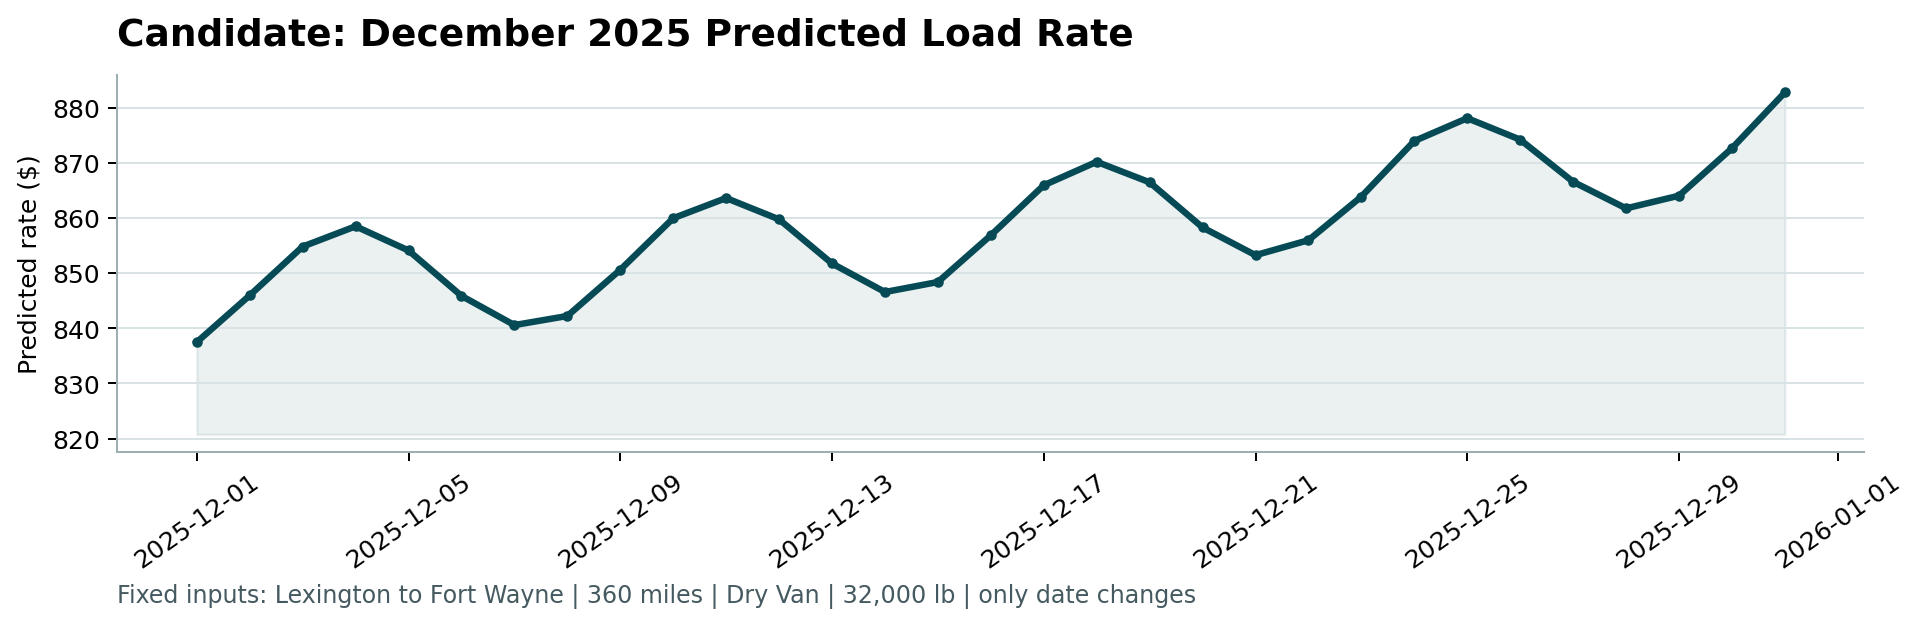
\includegraphics[width=0.9\textwidth]{scorer_results/candidate_december.png}
  \caption{December 2025 predicted rate for the fixed Lexington to Fort Wayne load, as drawn by \texttt{score.py}.}
  \label{fig:december}
\end{figure*}

\section{The December chart}\label{sec:december}
\balance

The chart rises from \$838 on 1~December to \$883 on 31~December, with a weekly wobble on top (Figure~\ref{fig:december}). It prices one fixed load (Lexington to Fort Wayne, 360 miles, Dry Van, 32,000\,lb) for every day of December, so only the date changes.

The chart rows don't include a market index, and the model needs one. For each December day I used the average market index of that day's loads in Spotter's own prediction set (only their inputs, never prices), so the chart reflects December's actual market rather than a guess.

Each part of the shape comes from something in the data:
\begin{itemize}
  \item The weekly ups and downs are the market index's own weekly cycle: high mid-week, low at the weekend.
  \item The steady climb is the upward drift (about +0.6\% a month) plus the quarter-end ramp. All of December falls in the last five weeks of the quarter, so the ramp builds through the whole month.
  \item The highest point is the last day, 31~December, where the Dry Van quarter-end surge peaks. September, the previous quarter end, was the model's most accurate test month, which is some reassurance about this part.
\end{itemize}

For scale, real Dry Van loads on this lane between January and October were priced between about \$760 and \$930, depending on weight and date.

\section{Limitations}\label{sec:limitations}

\begin{itemize}
  \item The drift is a straight line, so a sudden level shift like the one at the start of October is only partly captured. If prices step again in November or December, predictions would lag by around 1\% until the model is retrained.
  \item The eight unseen cities are priced from their neighbours. That worked well when tested (1.55\% error), but it is still less accurate than for cities the model has seen (about 1.37\%).
  \item The model takes the market index at face value: it assumes the index's link to price (about +1.5\% per +0.1) holds in November--December. The index stays inside its training range there (0.72--1.10), so this isn't an extrapolation.
  \item Most of what's left is noise. About 1.8\% of each price isn't explained by anything in the data, so there is little room below the current error with these inputs.
\end{itemize}

% ---------------------------------------------------------------- appendix
\onecolumn
\raggedbottom
\appendix
\titleformat{\section}{\normalfont\large\bfseries}{Appendix \thesection}{0.8em}{}
\titlespacing*{\section}{0pt}{3ex plus 0.6ex minus 0.3ex}{1.2ex plus 0.2ex}

\section{Data-quality issues in full}\label{app:data}

\begin{center}
\small
\begin{tabularx}{\textwidth}{@{}l r X l@{}}
  \toprule
  Issue & Loads (of 48,000) & What the evidence showed & Handling \\
  \midrule
  Posted rate off by 2--6$\times$ & 677 (1.4\%) & Every other load within 0.92--1.11$\times$ of expected; nothing in between & Removed from training and scoring \\
  Weight capped at 47,500\,lb & 1,204 (2.5\%) & Prices like the heaviest uncapped loads & Kept, flagged \\
  Market index missing & 374 (0.8\%) & Missing at random; mostly a daily value & Same day's average, flagged \\
  Weight missing & 300 (0.6\%) & Missing at random; prices like an average load & Training median, flagged \\
  Negative weight & 292 (0.6\%) & Absolute values price like normal weights & Sign flipped \\
  Distance at the 70-mile floor & 48 (0.1\%) & Very short lanes clamped & Kept \\
  Weight at the 5,000\,lb floor & 32 (0.1\%) & Light loads clamped & Kept \\
  \texttt{quote\_signal} & all & Link to price switches on and off by month & Left out of the model \\
  \bottomrule
\end{tabularx}
\end{center}

\Needspace*{20\baselineskip}
\section{What the final model learned}\label{app:learned}

The same model fitted twice: on January--August (the version scored on the test) and on January--October (the version that made the submission). The effects barely move between the two.

\begin{center}
\small
\begin{tabular}{@{}lrr@{}}
  \toprule
  Effect on price & Fitted on Jan--Aug & Fitted on Jan--Oct \\
  \midrule
  Reefer vs Dry Van & +12.5\% & +12.5\% \\
  Flatbed vs Dry Van & +7.5\% & +7.6\% \\
  Market index, per +0.1 & +1.6\% & +1.5\% \\
  Upward drift, per month & +0.5\% & +0.6\% \\
  Quarter-end surge on the last day: Dry Van & +2.6\% & +2.4\% \\
  Quarter-end surge on the last day: Reefer & +5.5\% & +5.2\% \\
  Quarter-end surge on the last day: Flatbed & +8.6\% & +8.5\% \\
  Weekday vs Monday & $-$0.6\% to 0\% & $-$0.5\% to 0\% \\
  City effects, lowest to highest & $-$3.7\% to +3.2\% & $-$3.7\% to +3.3\% \\
  Lane effects, typical size & $\pm$0.8\% & $\pm$0.8\% \\
  \bottomrule
\end{tabular}
\end{center}

The weekday effects are small because the weekly price cycle comes through the market index, which moves on the same weekly rhythm.

Settings: ridge penalty 0.01, with lane effects penalised 100$\times$ harder; distance curve with 8 knots, weight curve with 6; quarter-end ramp over 35 days with power 1.5; unseen cities use their 3 nearest known cities.

\Needspace*{20\baselineskip}
\section{Results in full}\label{app:results}

Loads exclude corrupted prices.

\begin{center}
\small
\begin{tabular}{@{}llrrrrr@{}}
  \toprule
  & & & \multicolumn{2}{c}{Baseline} & \multicolumn{2}{c}{Final model} \\
  \cmidrule(lr){4-5}\cmidrule(l){6-7}
  Split & Months scored & Loads & MAPE & \$ error & MAPE & \$ error \\
  \midrule
  Fold 1 & Apr--May & 9,604 & 1.90\% & \$47 & 1.37\% & \$34 \\
  Fold 2 & May--Jun & 9,571 & 1.60\% & \$39 & 1.34\% & \$34 \\
  Fold 3 & Jun--Jul & 9,567 & 1.61\% & \$39 & 1.27\% & \$31 \\
  Fold 4 & Jul--Aug & 9,538 & 1.82\% & \$43 & 1.48\% & \$35 \\
  Folds, average & & & 1.73\% & \$42 & 1.37\% & \$33 \\
  \midrule
  Test, September & Sep & 4,606 & 1.70\% & \$40 & 1.23\% & \$29 \\
  Test, October & Oct & 4,773 & 1.70\% & \$39 & 1.59\% & \$37 \\
  Test, overall & Sep--Oct & 9,379 & 1.70\% & \$39 & 1.41\% & \$33 \\
  \bottomrule
\end{tabular}
\end{center}

\Needspace*{20\baselineskip}
\section{Alternative models}\label{app:alternatives}

Same four folds, same cleaned data and feature table. The tree models and the neural network got every feature, including the date trend.

\begin{center}
\small
\begin{tabular}{@{}lrr@{}}
  \toprule
  Model & Fold MAPE & Worst fold \\
  \midrule
  Final model + LightGBM on what it leaves (hybrid) & 1.36\% & 1.47\% \\
  Final model & 1.37\% & 1.48\% \\
  Baseline: linear regression & 1.73\% & 1.90\% \\
  CatBoost & 2.01\% & 2.40\% \\
  LightGBM & 2.11\% & 2.19\% \\
  XGBoost & 2.13\% & 2.26\% \\
  Random forest & 2.97\% & 3.62\% \\
  Neural network (small MLP) & 4.88\% & 10.91\% \\
  Linear regression on raw dollars & 5.13\% & 5.43\% \\
  \bottomrule
\end{tabular}
\end{center}

The tree models drift into under-pricing the further ahead they predict, since they can't carry the upward trend past their training dates; a small LightGBM tuning round didn't change that. The neural network broke down in fold 1, where the market index climbed above anything it had trained on. The hybrid is level with the final model, so it wasn't worth a second model.

\Needspace*{14\baselineskip}
\section{How to reproduce}\label{app:reproduce}

\begin{lstlisting}
python -m pip install -r requirements.txt

# the submission: validation_predictions.csv and the December chart
python -m freight.predict
python score.py --predictions validation_predictions.csv --december-predictions data/december_chart_inputs.csv

# the fold and test results, and the tests
python -m freight.evaluate
python -m freight.evaluate --test
python -m pytest
\end{lstlisting}

The code lives in \code{freight/} (cleaning, features, validation, models, prediction), with the analysis in \code{notebooks/01_eda.ipynb} and \code{notebooks/02_modelling.ipynb}.

\end{document}
